\section{Anisotropic Strain-Gradient Continuum with Micro-Inertia}
\label{sec:continuum}

\subsection{Ellipsoidal characteristic-length tensor}
Isotropic gradient elasticity commonly uses one characteristic length $l$.For an oriented microstructure in plane strain, we now consider an in-plane averaging area $\mathcal{E}_0$ in the form of an ellipse of semi-axes $l_1$ and $l_2$ :
\begin{equation}
\mathcal{E}_0 = \left\{ (x_1', x_2') \in \mathbb{R}^2 \;\middle|\; \frac{(x_1')^2}{l_1^2} + \frac{(x_2')^2}{l_2^2} \le 1 \right\},
\label{eq:ellipse_def}
\end{equation}
The points $(x_1',x_2')$ are on the principal directions of the ellipse. The length tensor in these coordinates is defined by the squared semi-axes instead of the normalised covariance of a uniformly filled ellipse:
\begin{equation}
\mathbf{L}_0 = \begin{bmatrix} l_1^2 & 0 \\ 0 & l_2^2 \end{bmatrix}.
\label{eq:L0_mat}
\end{equation}

As the aspect ratio of the ellipse changes, the area of the ellipse remains fixed. With $l_{\mathrm{iso}}>0$ as the isotropic reference length, this condition gives:
\begin{equation}
\begin{split}
l_1 &= l_{\mathrm{iso}}\sqrt{\mathrm{AR}}, \quad l_2 = \frac{l_{\mathrm{iso}}}{\sqrt{\mathrm{AR}}}, \\
\pi l_1l_2 &= \pi l_{\mathrm{iso}}^2, \\
\det(\mathbf{L}_0) &= l_1^2l_2^2 = l_{\mathrm{iso}}^4 = \mathrm{const},
\end{split}
\label{eq:volume_equivalent}
\end{equation}
Here $\mathrm{AR}=l_1/l_2\ge1$. The second-moment factor of the three-dimensional averaging domain, an ellipsoidal solid, is $1/10$. This is a factor that is maintained throughout the process of the formulation, and in the case of the plane strain reduction. The law below is the scalar-length form used for the constitutive and stiffness expressions at $l_1=l_2$.

\subsubsection{Orientation convention and passive rotation}
We take positive $\theta$ to denote a clockwise orientation of the principal axes relative to the global frame $(x_1,x_2)$. The passive map from global coordinates $\bmx$ to local principal coordinates $\bmx'$ is:
\begin{equation}
\bmx' = \bmR(\theta)\bmx, \quad \bmR(\theta) = \begin{bmatrix} \cos\theta & -\sin\theta \\ \sin\theta & \cos\theta \end{bmatrix}.
\label{eq:R_matrix}
\end{equation}
Under this coordinate transformation, the characteristic-length tensor in the global frame is:
\begin{equation}
\setlength{\arraycolsep}{3pt}
\begin{split}
\mathbf{L}(\theta) &= \bmR(\theta)^\mathsf{T} \mathbf{L}_0 \bmR(\theta) \\
&= \begin{bmatrix} \cos\theta & \sin\theta \\ -\sin\theta & \cos\theta \end{bmatrix} \begin{bmatrix} l_1^2 & 0 \\ 0 & l_2^2 \end{bmatrix} \begin{bmatrix} \cos\theta & -\sin\theta \\ \sin\theta & \cos\theta \end{bmatrix}.
\end{split}
\label{eq:L_rotation}
\end{equation}
The tensor components are:
\begin{subequations}
\label{eq:L_components}
\begin{align}
L_{11}(\theta) &= l_1^2 \cos^2\theta + l_2^2 \sin^2\theta, \label{eq:L11} \\
L_{22}(\theta) &= l_1^2 \sin^2\theta + l_2^2 \cos^2\theta, \label{eq:L22} \\
L_{12}(\theta) &= L_{21}(\theta) = (l_2^2 - l_1^2)\cos\theta\sin\theta. \label{eq:L12}
\end{align}
\end{subequations}
For an elongated microstructure ($l_1 > l_2$), the off-diagonal coupling $L_{12}(\theta)$ is negative for $0 < \theta < 90^\circ$ and reaches its minimum, $(l_2^2-l_1^2)/2$, at $\theta=45^\circ$. Figure~\ref{fig:ellipsoid_tensor} shows the ellipses and the orientation dependence of $L_{11}$, $L_{22}$ and $L_{12}$. Because $\bmR(\theta)$ is orthogonal, the eigenvalues of $\mathbf{L}(\theta)$ are invariant under rotation:
\begin{equation}
\mathrm{spec}(\mathbf{L}(\theta)) \equiv \{l_1^2, l_2^2\} \quad \forall\,\theta \in [0, 2\pi).
\label{eq:eigenvalues_invariant}
\end{equation}
For $l_1,l_2>0$, $\mathbf{L}(\theta)$ is positive definite at every orientation.

\begin{figure*}[htbp]
\centering
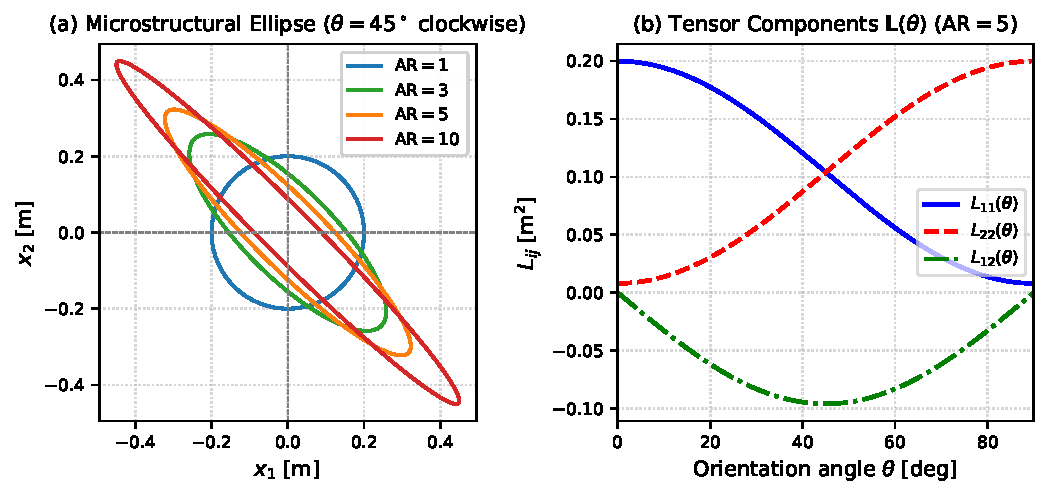
\includegraphics[width=\textwidth]{figures/fig01_ellipsoid_tensor.pdf}
\caption{Length-scale anisotropy. (a) Equal-area ellipses at $\theta=45^\circ$. (b) Length-tensor components against orientation for $\mathrm{AR}=5$.}
\label{fig:ellipsoid_tensor}
\end{figure*}

\subsection{Kinematics and constitutive response}
We assume infinitesimal deformations and two-dimensional plane-strain conditions ($u_3 = 0, \partial(\cdot)/\partial x_3 = 0$). The classical displacement gradient gives the infinitesimal strain tensor $\bm\varepsilon$:
\begin{equation}
\varepsilon_{ij} = \frac{1}{2}(u_{i,j} + u_{j,i}), \quad i,j \in \{1, 2\}.
\label{eq:strain_def}
\end{equation}
The strain-gradient tensor $\bm\eta$ is the spatial derivative of the strain:
\begin{equation}
\eta_{ijk} = \varepsilon_{ij,k} = \frac{1}{2}(u_{i,jk} + u_{j,ik}), \quad \eta_{ijk} = \eta_{jik}.
\label{eq:strain_gradient_def}
\end{equation}
Under plane strain in 2D, $\bm\varepsilon$ has 3 independent components ($\varepsilon_{11}, \varepsilon_{22}, 2\varepsilon_{12}$), and $\bm\eta$ has 6 ($\eta_{111}, \eta_{112}, \eta_{221}, \eta_{222}, 2\eta_{121}, 2\eta_{122}$).

\subsubsection{Mindlin Form-II constitutive law}
In Mindlin's Form II, the strain-energy density $W$ has classical and strain-gradient contributions:
\begin{equation}
W = \frac{1}{2}\sigma_{ij}\varepsilon_{ij} + \frac{1}{2}\tau_{ijk}\eta_{ijk},
\label{eq:strain_energy_W}
\end{equation}
where $\bm\sigma$ is the Cauchy stress tensor and $\bm\tau$ is the third-order double-stress (or dipolar stress) tensor. For an isotropic base material parameterised by the Lam\'e constants $\lambda$ and $\mu$, the Cauchy stress satisfies Hooke's law:
\begin{equation}
\sigma_{ij} = C_{ijkl}\varepsilon_{kl} = \lambda \delta_{ij}\varepsilon_{kk} + 2\mu \varepsilon_{ij}.
\label{eq:cauchy_stress}
\end{equation}
The double-stress tensor $\tau_{ijk}$ is conjugate to $\eta_{ijk}$ through the anisotropic gradient-elasticity law with $\mathbf{L}$:
\begin{equation}
\begin{split}
\tau_{ijk} &= \frac{1}{10} L_{kl} C_{ijmn}\eta_{mnl} \\
&= \frac{1}{10} L_{kl}\left(\lambda \delta_{ij}\eta_{mml} + 2\mu \eta_{ijl}\right),
\end{split}
\label{eq:double_stress}
\end{equation}
For stable isotropic elastic constants ($\mu>0$ and $3\lambda+2\mu>0$) and positive-definite $\mathbf{L}$, the quadratic strain energy is non-negative and vanishes only when the strain and strain-gradient fields both vanish.

\subsubsection{Gradient micro-inertia}
We include gradient micro-inertia in the kinetic-energy density $T$:
\begin{equation}
T = \frac{1}{2}\rho \dot u_i \dot u_i + \frac{1}{2}\rho \ell_{\mathrm{i}}^2 \dot u_{i,j}\dot u_{i,j},
\label{eq:kinetic_energy_T}
\end{equation}
where $\rho$ is the macroscopic mass density and $\ell_{\mathrm{i}} > 0$ is the independent micro-inertia length parameter. Applying Hamilton's principle $\delta \int_{t_1}^{t_2} (T - W)\,\dif t = 0$ gives the strong-form equations of dynamic equilibrium in the bulk:
\begin{equation}
\sigma_{ij,j} - \tau_{ijk,jk} = \rho\left(\ddot u_i - \ell_{\mathrm{i}}^2 \ddot u_{i,jj}\right), \quad \text{in } \Omega.
\label{eq:strong_form}
\end{equation}
The operator $1-\ell_{\mathrm{i}}^2\nabla^2$ increases the effective inertia of spatially varying acceleration. It gives the transverse branch a finite high-wavenumber phase-speed limit, as derived in Appendix~\ref{app:asymptotics}.

\subsubsection{Model reductions}
The model has four useful physical limits:
\begin{enumerate}[label=(\roman*)]
  \item \textbf{Classical elasticity limit ($l_{\mathrm{iso}} \to 0$ at fixed finite $\mathrm{AR}$, $\ell_{\mathrm{i}} \to 0$):} Both principal gradient lengths and the double stresses vanish, and the classical Navier equations $\sigma_{ij,j}=\rho\ddot u_i$ are recovered with dispersionless acoustic speeds $c_T=\sqrt{\mu/\rho}$ and $c_L=\sqrt{(\lambda+2\mu)/\rho}$.
  \item \textbf{Isotropic gradient elasticity ($\mathrm{AR} = 1$):} Here $l_1 = l_2 = l_{\mathrm{iso}}$, so $L_{11} = L_{22} = l_{\mathrm{iso}}^2$ and $L_{12} = 0$ for all $\theta$, recovering isotropic Form-II gradient elasticity.
  \item \textbf{Gradient elasticity without micro-inertia ($\ell_{\mathrm{i}} = 0$):} The higher order stiffness is reserved, while the inertial correction is gone. For the transverse branch, $v_p\propto k$ as $k\to\infty$.
  \item \textbf{Quarter-turn covariance:} For fixed $l_1,l_2$, a $90^\circ$ change of orientation interchanges the diagonal components and reverses the sign of the off-diagonal component: $L_{11}(\theta+90^\circ)=L_{22}(\theta)$, $L_{22}(\theta+90^\circ)=L_{11}(\theta)$, and $L_{12}(\theta+90^\circ)=-L_{12}(\theta)$.
\end{enumerate}

\subsection{Boundary operators}
Suppose that the boundary $\Gamma=\partial\Omega$ is smooth and has the unit outward normal $\bm n$. The boundary contribution comes from the strain-energy term integrated by parts.
\begin{equation}
\begin{split}
\left.\delta\int_\Omega W\,\dif\Omega\right|_\Gamma
={}& \int_\Gamma \Big[(\sigma_{ij}-\tau_{ijk,k})n_j\,\delta u_i \\
&+ \tau_{ijk}n_k\,\delta u_{i,j}\Big] \,\dif\Gamma.
\end{split}
\label{eq:elastic_boundary_work}
\end{equation}
On a smooth boundary, we decompose $\delta u_{i,j}$ into normal and tangential parts. Integrating the tangential part by parts then gives the work-conjugate double traction and the effective elastic traction:
\begin{equation}
\begin{split}
R_i &= n_jn_k\tau_{ijk}, \\
p_i^{\mathrm{el}} &= (\sigma_{ij}-\tau_{ijk,k})n_j - \nabla_j^S(n_k\tau_{ijk}),
\end{split}
\label{eq:traction_def}
\end{equation}
where $\nabla_j^S$ denotes the surface divergence on the tangential component of $n_k\tau_{ijk}$. Additional line forces arise at boundary edges. The gradient micro-inertia adds $\rho\ell_{\mathrm{i}}^2\ddot u_{i,j}n_j$ to the dynamic traction, so $p_i^{\mathrm{dyn}}=p_i^{\mathrm{el}}+\rho\ell_{\mathrm{i}}^2\ddot u_{i,j}n_j$. The work-conjugate pairs are $(u_i,p_i^{\mathrm{dyn}})$ and $(\partial u_i/\partial n,R_i)$. The paired cell faces carry Bloch phase conditions instead of independent free-boundary conditions.
